	\pagecolor{goban}
\thispagestyle{empty}
\begin{center}
	\vspace*{1cm} 
	\begin{tikzpicture}
		\node[font=\fontsize{180}{156}\bfseries\selectfont, text=black] at (0,0) {圍道};
		
	\end{tikzpicture}
	%		\begin{tikzpicture}
		%			\node[font=\fontsize{196}{156}\bfseries\selectfont, text=black] at (0,0) {圍};
		%			\node[font=\fontsize{196}{156}\bfseries\selectfont, text=black] at (0,-8) {道};
		%		\end{tikzpicture}
	\vspace{1.5cm}
	
	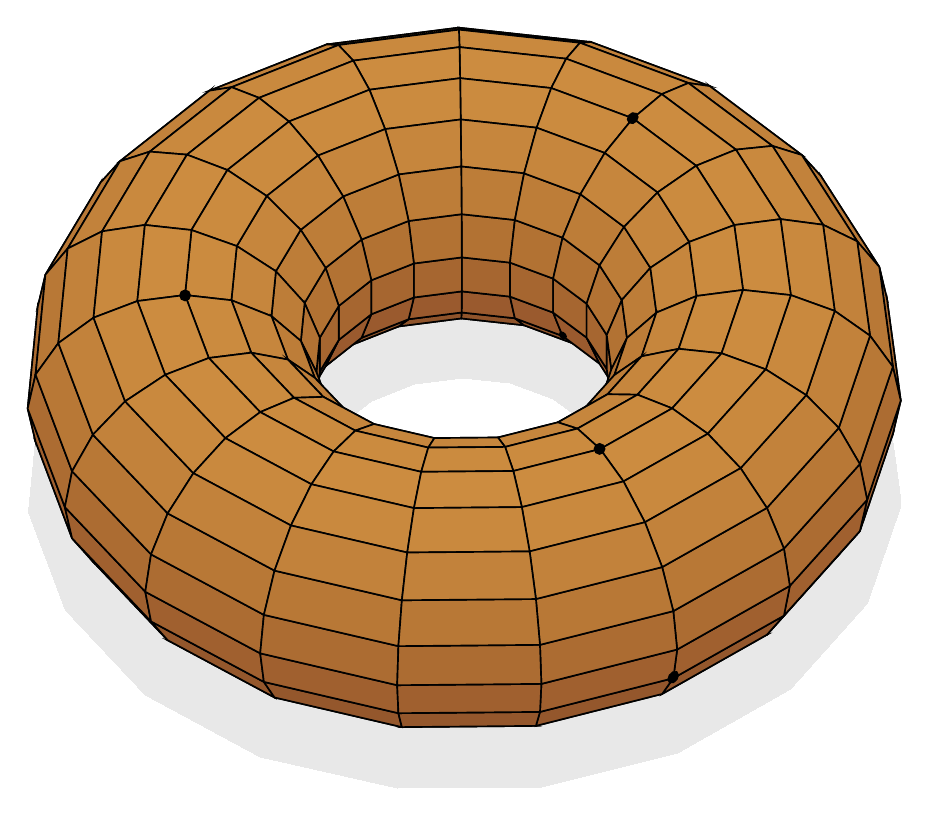
\begin{tikzpicture}[scale=3]
		\pgfplotsset{
			colormap={teak}{
				rgb=(0.5,0.3,0.15)
				rgb=(0.6,0.35,0.18)
				rgb=(0.7,0.45,0.2)
				rgb=(0.8,0.55,0.25)
			},
			% New colormap specifically for the shadow
			colormap={shadow}{
				gray=(0.1)
				gray=(0.1)
			}
		}
		\begin{axis}[
			hide axis,
			view={4}{45},
			axis equal image,
			samples=20,
			domain=0:360,
			y domain=0:360,
			z buffer=sort,
			]
			
			% 1. Sombra
			\addplot3[
			surf,
			shader=interp,
			draw=none,     
			colormap name=shadow,
			opacity=0.1
			]
			(
			{(2 + cos(y)) * cos(x)},
			{(2 + cos(y)) * sin(x)},
			{-1} 
			);
			
			% 2. toro
			\addplot3[
			surf,
			shader=flat,
			draw=black,
			colormap name=teak,
			line width=0.2pt,
			opacity=1
			]
			(
			{(2 + cos(y)) * cos(x)},
			{(2 + cos(y)) * sin(x)},
			{sin(y)}
			);
			
			%%%%%%%%%%%%%%%%%%%%  puntos negros
			\addplot3[
			only marks,
			xslant=-0.15,
			yslant=-0.5,
			mark options={shading=ball, ball color=white},
			mark size=0.25pt,
			shading=ball,
			color=black
			] coordinates {(1.190, 3.94, 0)};
			
			\addplot3[
			only marks,
			mark options={shading=ball, ball color=white},
			mark size=0.5pt,
			shading=ball,
			color=black
			] coordinates {(-1.96, 0.675, 0)};
			
			\addplot3[ %centro
			only marks,
			mark options={shading=ball, ball color=white},
			mark size=0.5pt,
			shading=ball,
			color=black
			] coordinates {(0.975, -0.61, 0)};
			
			\addplot3[ %arriba derecha
			only marks,
			yslant=0.25,
			mark options={shading=ball, ball color=white},
			mark size=0.5pt,
			shading=ball,
			color=black
			] coordinates {(1.09, 1, 0)};
			
			\addplot3[ %abajo derecha
			only marks,
			yslant=0.5,
			mark options={shading=ball, ball color=black},
			mark size=0.5pt,
			shading=ball,
			color=black
			] coordinates {(1.870,-6.179, 0)};
		\end{axis}
	\end{tikzpicture}
	\vspace{1cm}
	
	% 2. Aplicación de la fuente al título
	
\begin{tikzpicture}
		% Changes the node to Helvetica
		\node[font=\fontspec{EBGaramond-Bold.ttf}\fontsize{24}{156}\bfseries\selectfont, text=black!90] at (0,-1) {The art of surrounding};
		%\node[font=\fontspec{EBGaramond-Bold.ttf}\fontsize{16}{156}\bfseries\selectfont, text=black!80] at (0,-2) {Arias, W. Adrián};
	\end{tikzpicture}
	
	
\end{center}
\newpage
%%%%%%%%% PORTADA

\pagecolor{white}
\thispagestyle{empty}
\clearpage

\thispagestyle{empty}
\maketitle
% --- FORZAR ESTILO EN PÁGINAS DE CAPÍTULO ---
% Redefinimos el estilo 'plain' que LaTeX usa automáticamente al iniciar capítulos
\clearpage
\thispagestyle{empty}

\vspace*{0.2925\textheight} % Ajuste para el »Centro Óptico» (más arriba que el centro)

\begin{center}
	% Usamos un ancho similar al del bloque del poema (ej. 7.5cm o 8cm)
	% para que el »peso» visual del cuadrado de la foto sea igual al del texto.
	%		
\includegraphics[width=7.5cm]{ipe_mitad.jpg}
	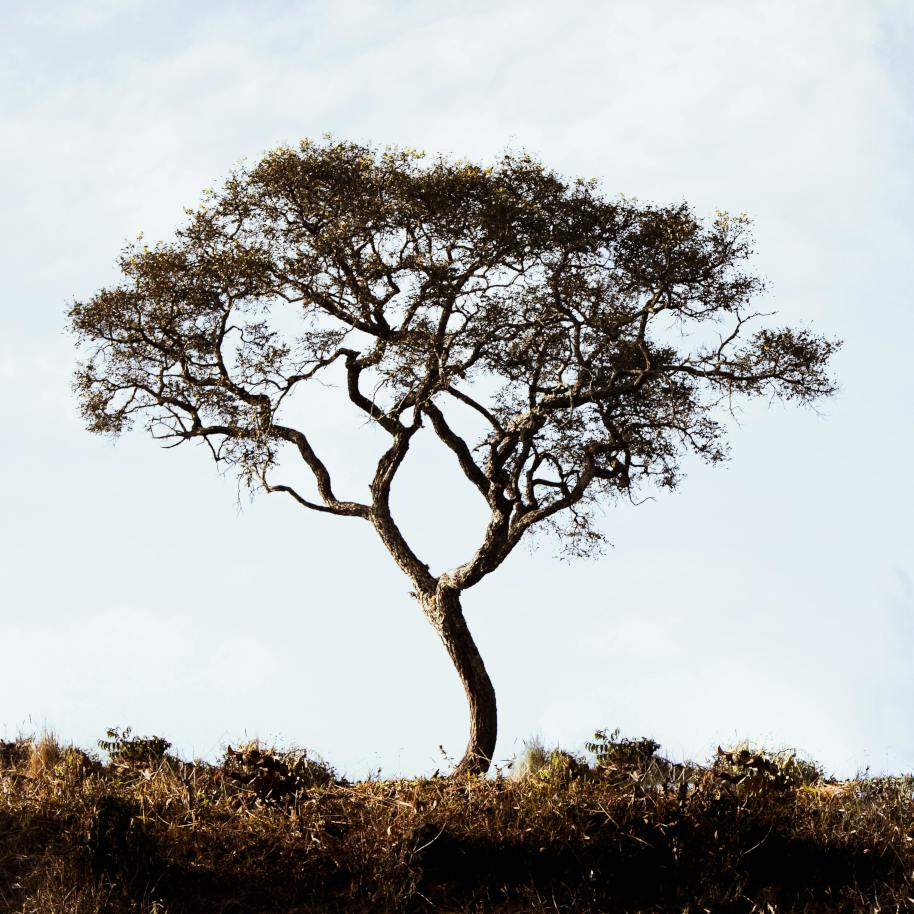
\includegraphics[width=7.5cm]{figures/ipe_cuarto.jpg}
\end{center}

\vspace*{\fill} % Empuja desde abajo
\clearpage
\thispagestyle{empty} % Esto quita encabezados, pies y números de esta página
\vspace*{0.3\textheight} % Ajuste para el »Centro Óptico» (más arriba que el centro)

\begin{center}
	\begin{minipage}{6.375cm}
		\linespread{1.3}\selectfont
		\itshape
		Contemplo o rio que corre parado \\
		E a dançarina de pedra que evolui \\
		Completamente, sem metas, sentado \\
		Não tenho sido, não sou, não serei, nem fui \\
		A mente quer ser, mas querendo erra \\
		Pois só sem desejos é que se vive o agora\\
		Vêde o pé do ypê, apenasmente flora\\
		Revolucionariamente\\
		Apenso ao pé da serra
		
		\vspace{1.5em}
		\hfill \upshape  --- \textbf{Belchior} «Ypê»
	\end{minipage}
\end{center}
\vfill % Empuja todo hacia arriba
\clearpage
\thispagestyle{empty}
\section*{Preface}
\thispagestyle{empty}
What's Go? A game, of course. But one might ask: How is it done precisely? What can be done and what not? Is it possible to extend its concepts to other games?

\textit{圍道 — Wéi Dào — The art of surrounding} Tries to answer such questions by constructing a rigorous theory of the game of Go, followed by its generalization on and out of the board.

This work is separated into three parts as follows:

\textbf{Part I: Foundation.} We begin the study of the game by its history, starting in ancient China to its development in Argentina. We finish this part with the rules of the game and setting the construction motivation.

\textbf{Part II: Construction.} Now that we know the game, we are ready to build it formally. The two-dimensional version of the game is constructed. The board, the pieces, the colors, and the relations between them are defined. Followed by the concepts of group, captures, and SuperKo. The legality of a play is formalized via a theorem. The SuperKo detection is handled by Zobrist Hashing. The whole structure is named Go, and we begin to generalize it. Later, we discuss the \textit{life in the game of Go} also know as \textit{inconditional life} by interpretating, in this theory, the results of David Benson; also, we develop the theory around the \textit{conditional life} (Briefly, WIP). At the very end we discuss about two papers from Kim Jin Bai, in the second one of those there is a theorem that uses Benson results and we develop a counter-example of a Theorem.

\textbf{Part III: Abstraction.} We now study the board from outside, taking in consideration a little intuiton about the three dimensional Go, a concept about the quantity of liberties of a board naturally appears, such concept leads to a problem about liberties and how to control how the growth whenever the board get's big (in dimension). We also attack the one dimensional Go and finally we try to look beyond The game of Go in order to find if the structure we have made up for it can suit up other games.

\vfill

I would like to thank Gusti Cabaña for being my first reader and giving me direction when I needed it most. Thanks also go to Diego Barrios and Eros Girardi for reviewing this work and providing invaluable feedback. Lastly, to Naza, for putting up with me throughout all these years and the years to come.

Lastly I'd like to acknowledge that the very first installment of this ``Book'' was made for a monograph competition. This it just for future reference of how important such competition might be for the development of mathematics or, at the very least, the mathematical spirit within oneself.
\clearpage

\tableofcontents
\thispagestyle{empty}
\clearpage